\begin{figure}[t]
	\centering
	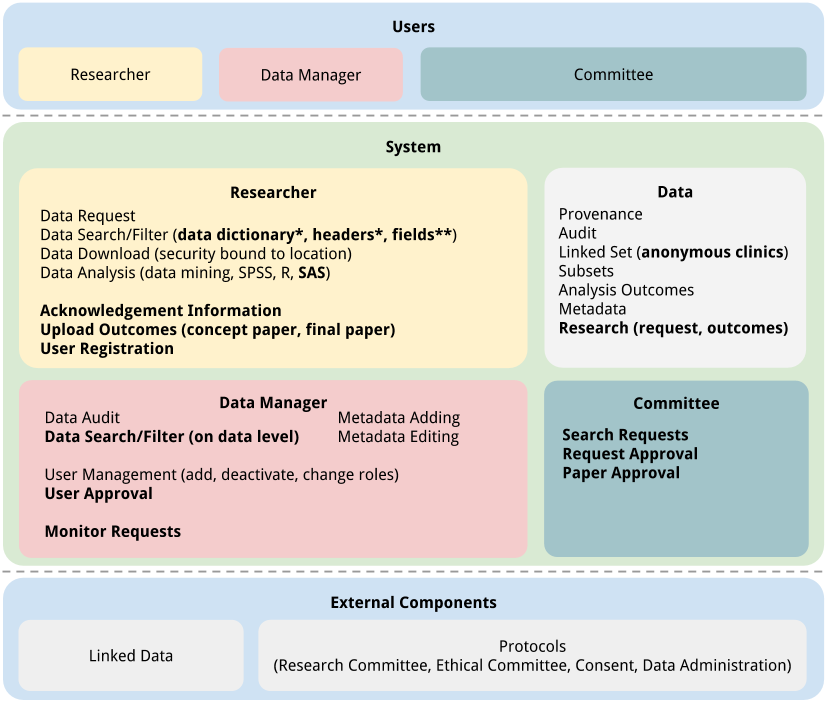
\includegraphics[width=1.0\linewidth]{images/brainstorm-after}
	\caption{
		\ivfsystem{} schema after brainstorm, encompassing data, user, request, and publication management.
		The system offers different sets of functions for three user roles (researcher, data manager, and committee) indicated by colours. 
		External components are (offline) essential parts for system (\eg{} data, regulations) but are outside the scope of development (and by extension of this study).
		Data listed is either available at initialisation of the system or is generated during execution.
		*: The data dictionary contains information about all the available data items, also called: headers.
		\allard{needs to be clear that data is stored as a table, where data is stored in rows and columns, the column names are called headers here}
		**: Fields are the `raw' data that belong to a stored pregnancy, fields are named with headers.
	}
	\label{fig:brainstorm-after}
\end{figure}

\paragraph{Final concept}

After the identification of the differences that were observed during the brainstorm session the final concept can be defined.
This section describes how the initial concept was transformed to form the final concept.

The final concept in this project is to develop a system for the \projectdata{} with capability for management for: users, requests, data, and publications.
While the functions in the initial concept were educated guesses, now they are validated by the brainstorm session.
Figure \ref{fig:brainstorm-after} describes the full view of the concept, which folds back into the function groups as shown in figure \ref{fig:research-workflow-after}.

Three direct users are planned each have their own set of functions with the data they use and produce.
The (offline) external components remain nearly unchanged, only the unlinked data has been removed, the protocols are still vital for the system.

A few changes were made to the system's data.
The linked set had to be made anonymous considering the clinic, meaning that clinics would not be directly comparable against each other.
Also data about the request and publications is now stored in the system, these are both captured in a `research'.

A lot of differences exist between the schema before and after the brainstorm, an side-by-side comparison is supplied in appendix \ref{brainstorm-before-after}.
The main assumption of a data support system had the wrong focus, it is now supplemented with increased request management and the addition of user and publication management.
While data handling functions like searching, security restriction, auditing, or annotating with metadata are important in this system there are more side effects of research that have to be taken into account.